
%%%%%%%%%%%%%%%%%%%%%%%%%%%%%%%%%%%%%%%%%%%%%%%%%%%%%%%%%%%%%%%%%%%%%%%%%%%%%%%%%%%%%%%
%%%%%%%%%%%%%%%%%%%%%%%%%%%%%%%%%%%%%%%%%%%%%%%%%%%%%%%%%%%%%%%%%%%%%%%%%%%%%%%%%%%%%%%
% 
% This top part of the document is called the 'preamble'.  Modify it with caution!
%
% The real document starts below where it says 'The main document starts here'.

\documentclass[12pt]{article}
\usepackage{hyperref}

\usepackage{amssymb,amsmath,amsthm}
\usepackage[top=1in, bottom=1in, left=1.25in, right=1.25in]{geometry}
\usepackage{fancyhdr}
\usepackage{enumerate}
\usepackage{listings}
\usepackage{graphicx}
\usepackage{float}
\usepackage{multicol}
% Comment the following line to use TeX's default font of Computer Modern.
\usepackage{times,txfonts}
\usepackage{mwe}
\usepackage{caption}
\usepackage{subcaption}

\usepackage{tikz}
\def\checkmark{\tikz\fill[scale=0.4](0,.35) -- (.25,0) -- (1,.7) -- (.25,.15) -- cycle;} 



\makeatletter
\renewcommand*\env@matrix[1][*\c@MaxMatrixCols c]{%
  \hskip -\arraycolsep
  \let\@ifnextchar\new@ifnextchar
  \array{#1}}
\makeatother

\newtheoremstyle{homework}% name of the style to be used
  {18pt}% measure of space to leave above the theorem. E.g.: 3pt
  {12pt}% measure of space to leave below the theorem. E.g.: 3pt
  {}% name of font to use in the body of the theorem
  {}% measure of space to indent
  {\bfseries}% name of head font
  {:}% punctuation between head and body
  {2ex}% space after theorem head; " " = normal interword space
  {}% Manually specify head
\theoremstyle{homework} 

% Set up an Exercise environment and a Solution label.
\newtheorem*{exercisecore}{\@currentlabel}
\newenvironment{exercise}[1]
{\def\@currentlabel{#1}\exercisecore}
{\endexercisecore}

\newcommand{\localhead}[1]{\par\smallskip\noindent\textbf{#1}\nobreak\\}%
\newcommand\solution{\localhead{Solution:}}

%%%%%%%%%%%%%%%%%%%%%%%%%%%%%%%%%%%%%%%%%%%%%%%%%%%%%%%%%%%%%%%%%%%%%%%%
%
% Stuff for getting the name/document date/title across the header
\makeatletter
\RequirePackage{fancyhdr}
\pagestyle{fancy}
\fancyfoot[C]{\ifnum \value{page} > 1\relax\thepage\fi}
\fancyhead[L]{\ifx\@doclabel\@empty\else\@doclabel\fi}
\fancyhead[C]{\ifx\@docdate\@empty\else\@docdate\fi}
\fancyhead[R]{\ifx\@docauthor\@empty\else\@docauthor\fi}
\headheight 15pt

\def\doclabel#1{\gdef\@doclabel{#1}}
\doclabel{Use {\tt\textbackslash doclabel\{MY LABEL\}}.}
\def\docdate#1{\gdef\@docdate{#1}}
\docdate{Use {\tt\textbackslash docdate\{MY DATE\}}.}
\def\docauthor#1{\gdef\@docauthor{#1}}
\docauthor{Use {\tt\textbackslash docauthor\{MY NAME\}}.}
\makeatother

% Shortcuts for blackboard bold number sets (reals, integers, etc.)
\newcommand{\Reals}{\ensuremath{\mathbb R}}
\newcommand{\Nats}{\ensuremath{\mathbb N}}
\newcommand{\Ints}{\ensuremath{\mathbb Z}}
\newcommand{\Rats}{\ensuremath{\mathbb Q}}
\newcommand{\Cplx}{\ensuremath{\mathbb C}}
%% Some equivalents that some people may prefer.
\let\RR\Reals
\let\NN\Nats
\let\II\Ints
\let\CC\Cplx

%\textbf{Code:}
%\begin{center}
%  \lstinputlisting{NewtonsMethodP5.m}
%\end{center}
%
%\textbf{Console:}
%\begin{center}
%  \lstinputlisting{P5C.txt}
%\end{center}
%\vspace{.15in}


%\begin{figure}[H]
%  \begin{center}
%    \caption{The one-norm unit ball}
%    \includegraphics[width=.76\textwidth]{1norm.png}
%  \end{center}
%\end{figure}




%%%%%%%%%%%%%%%%%%%%%%%%%%%%%%%%%%%%%%%%%%%%%%%%%%%%%%%%%%%%%%%%%%%%%%%%%%%%%%%%%%%%%%%
%%%%%%%%%%%%%%%%%%%%%%%%%%%%%%%%%%%%%%%%%%%%%%%%%%%%%%%%%%%%%%%%%%%%%%%%%%%%%%%%%%%%%%%
% 
% The main document start here.

% The following commands set up the material that appears in the header.
\doclabel{Math 615: Homework 4}
\docauthor{Stefano Fochesatto}
\docdate{\today}


\begin{document}


\begin{exercise}{Problem P18}
  \begin{enumerate}
    \item[(a)] Consider the following BFP with Dirichlet boundary conditions:
    \begin{equation*}
      u''(x) + u(x) = 0 \qquad \text{for,}\qquad a < x < b, \qquad u(a) = \alpha,\qquad u(b) = \beta
    \end{equation*}
    Write a Matlab, finite difference code to solve this problem. 
    \solution With a small modification to the code we wrote for P15 we get a three point centered finite difference scheme 
    to solve this problem. \\
    \textbf{Code:}
    \begin{center}
      \lstinputlisting[basicstyle = \footnotesize]{r1.txt}
    \end{center}

    \item[(b)] Determine the exact solution to the problem when $a = 0$, $b = 1$, $\alpha = 2$, and $\beta = 3$. 
    test your code from part (a) using this solution, including a demonstration of convergence at the optimal rate (which is what?)
    as $h \to 0$. Generate a convergence figure. 
    \solution Solving this problem by hand, first we form the characteristic equation, 
    \begin{equation*}
      r^2  + 1 = 0
    \end{equation*}
    Which gives roots $r = \pm i$. So we get the following general solution, 
    \begin{equation*}
      u(x) = c_1e^{ix} + c_2e^{-ix}. 
    \end{equation*} 
    Applying Euler's Formula we get 
    \begin{equation*}
      u(x) = c_1(\cos(x) + i\sin(x)) + c_2(\cos(x) - i\sin(x)).
    \end{equation*}
    Combining like terms and redefining our coefficient terms we get the general solution, 
    \begin{equation*}
      u(x) = c_1 \cos(x)  + c_2 \sin(x).
    \end{equation*}
    Solving the IVP with $u(0) = 2$ and $u(1) = 3$, we get the following, 
    \begin{align*}
      c_1 &= 2, \\
      c_2 &=  \frac{3 - 2\cos(1)}{\sin(1)}.
    \end{align*}
    So our solution looks like, 
    \begin{equation*}
      u(x) =  2\cos(x) + \frac{3 - 2\cos(1)}{\sin(1)}\sin(x)
    \end{equation*}

    Testing our code using this solution we get a convergence rate of $O(h^p)$ where $p \approx 2.001056$. Which is 
    as exprected with the optimal convergence rate of $O(h^2)$. Below is the convergence figure and code, we see 
    the optimal convergence graphed in purple, and our experimental convergence graphed in with circles. \\

      \begin{figure}[H]
        \begin{center}
          \caption{Convergence Plot via Discrete $L^2$ Norm}
          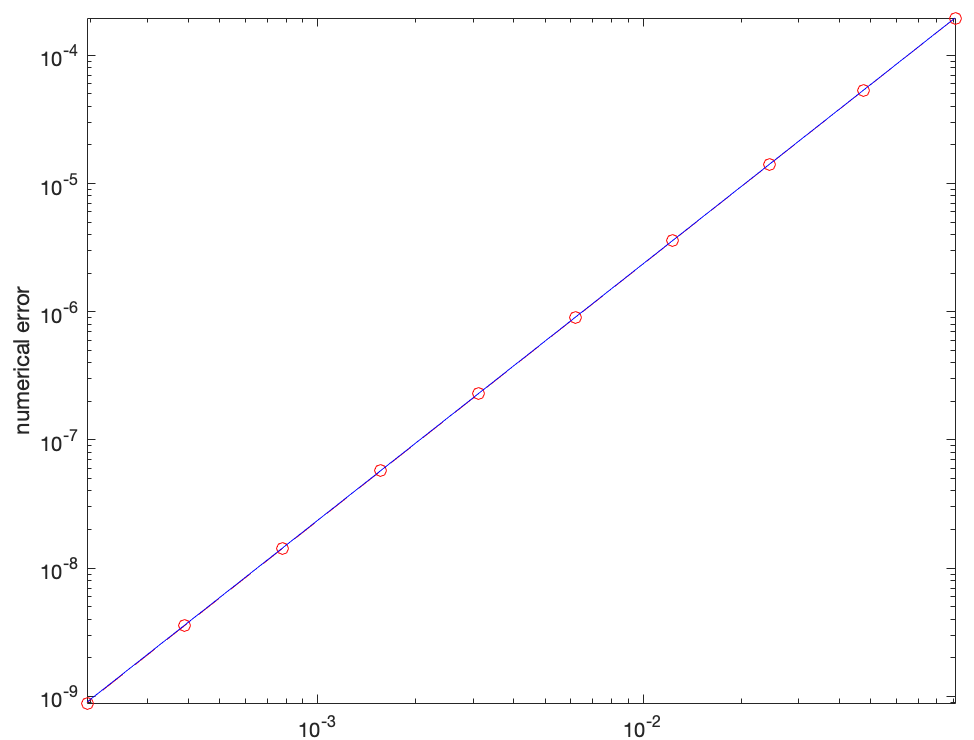
\includegraphics[width=.80\textwidth]{convergence.png}
        \end{center}
      \end{figure}

      \textbf{Console:}
      \begin{center}
        \lstinputlisting[basicstyle = \footnotesize]{r2.txt}
      \end{center}
      \vspace{.15in}

      \item[(c)] Let $a = 0$ and $b = \pi$. For what values of $\alpha$ and $\beta$ does $BVP$(1) have solutions?
      sketch a family of solutions in a case where there are infinitely-many solutions. \\
      \solution Recall that the general solution to $BVP$(1) is given by, 
      \begin{equation*}
        u(x) = c_1 \cos(x)  + c_2 \sin(x).
      \end{equation*}
      Note that $a = 0$ and $b = \pi$ generates the following system, 
      \begin{equation*}
        \begin{pmatrix}
          1 & 0\\
          -1 & 0
        \end{pmatrix}
        \begin{pmatrix}
          c_1\\
          c_2
        \end{pmatrix}
         = \begin{pmatrix}
          \alpha\\
          \beta
         \end{pmatrix}.
      \end{equation*}
      For this system to have a solution $\alpha = -\beta$, with $c_2$ as a free variable. The following is a plot of 
      a family of solution when $\alpha= C_1 = 1$  and $C_2$ is allowed to vary.
      \begin{figure}[H]
        \begin{center}
          \caption{Family of Solutions for BVP(1) with $a = 0$, $b = \pi$, and $\alpha = c_1 = 1$.}
          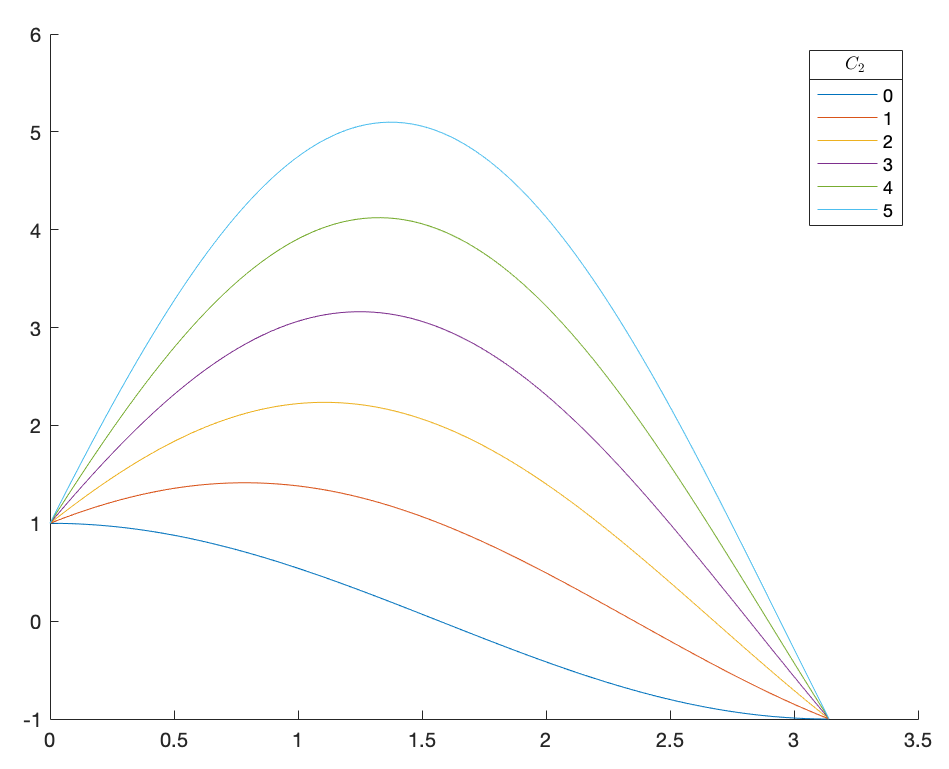
\includegraphics[width=.90\textwidth]{Family.png}
        \end{center}
      \end{figure}


      \textbf{Console:}
      \begin{center}
        \lstinputlisting[basicstyle = \footnotesize]{r3.txt}
      \end{center}

  \end{enumerate} 
  
\end{exercise}
\vspace{1in}



\begin{exercise}{Problem P19} Write a program to solve the BVP for the nonlinear pendulum as discussed in 
  the text, i.e. problem (2.77), using the Newton iteration strategy outlined in subsection 2.16.1. Reproduce Figures 2.4(b)
  and 2.5, for which $T = 2\pi$, and $\alpha = \beta = .7$.


  \solution Recall that the nonlinear BVP described in the text is, 
  \begin{align*}
    \theta''(t) = sin(&\theta(t)) \qquad \text{for } 0 < t < T\\
    \theta(0) = \alpha &\qquad \theta(T) = \beta 
  \end{align*}

  The Newton iteration strategy described in the text involves using a centered finite difference approximation for the $\theta''(t)$
  term to create a system of non-linear equations, 
  \begin{equation*}
    \frac{1}{h^2}(\theta_{i - 1} - 2\theta_i + \theta_{i + 1}) + \sin(\theta_i) = 0.
  \end{equation*}
  Note that this system is defined in $m$ dimensions using the same discretization scheme with $m+2$ equally spaced points between 0 and $T$ as we've used before. 
  To formulate the newton step we need to generate the Jacobian,    
  \begin{equation*}
    J = \frac{1}{h^2}
    \begin{bmatrix}
         (-2 + h^2\cos(\theta_1)) &    1    &         &             \\ 
               1 & (-2 + h^2\cos(\theta_2)) &    1    &              \\ 
                          &  \ddots &  \ddots & \ddots        \\
                                   &         &    1    & (-2 + h^2\cos(\theta_m)) 
    \end{bmatrix}.
  \end{equation*}
  The following code solves the double pendulum BVP problem via this Newton iteration strategy.\\ 
  
  \textbf{Code:}
  \begin{center}
    \lstinputlisting[basicstyle = \footnotesize]{r4.txt}
  \end{center}
Generating figure 2.4(b) from the text using initial iterate $\theta_i^{[0]} = .7$, $T = 2\pi$ and,  $\alpha = \beta = .7$

\begin{figure}[H]
  \begin{center}
    \caption{Figure 2.4b from the text. Note $k$ denotes iterate.}
    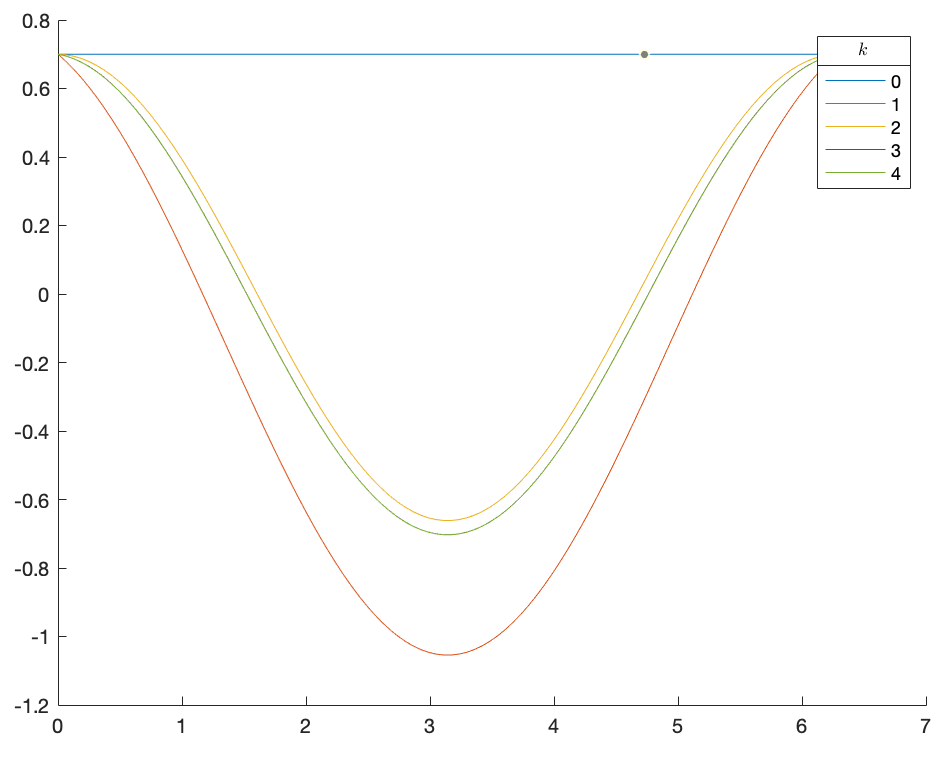
\includegraphics[width=.90\textwidth]{24b.png}
  \end{center}
\end{figure}


\textbf{Console:}
\begin{center}
  \lstinputlisting[basicstyle = \footnotesize]{r5.txt}
\end{center}

Generating figure 2.5 from the text using initial iterate $\theta_i^{[0]} = .7 + \sin(t_i/2)$, $T = 2\pi$ and,  $\alpha = \beta = .7$


\begin{figure}[H]
  \begin{center}
    \caption{Figure 2.5 from the text. Note $k$ denotes iterate.}
    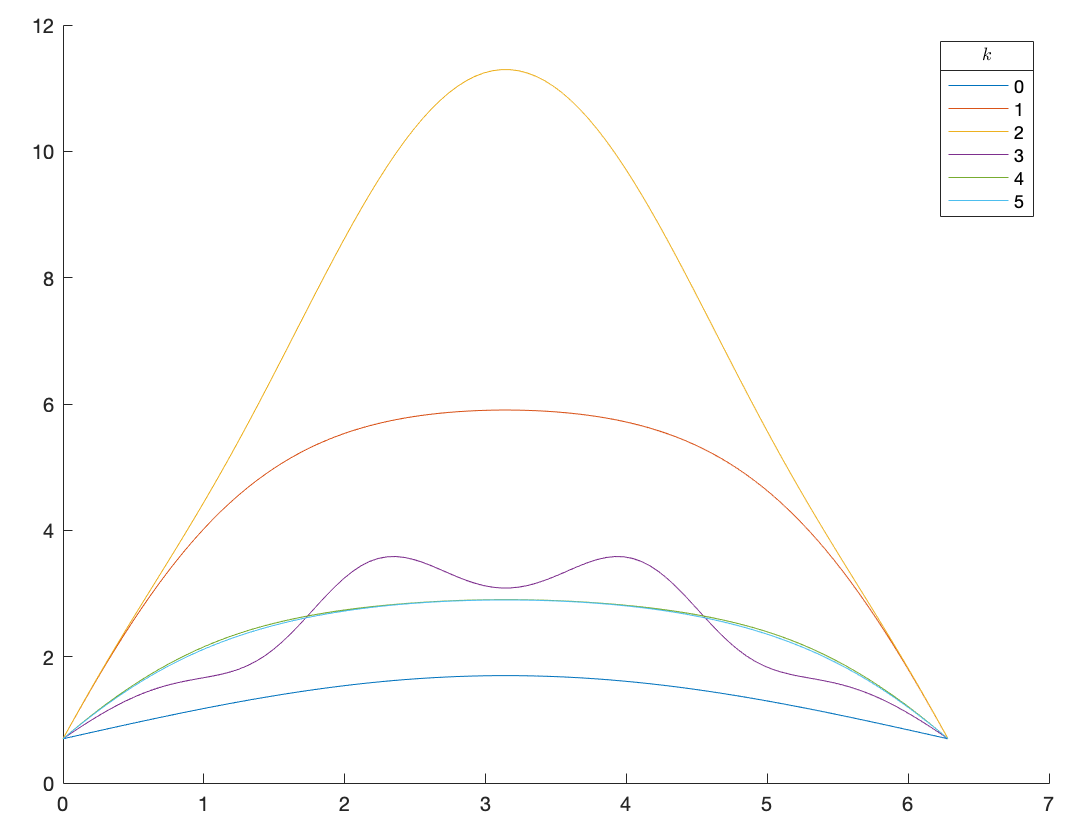
\includegraphics[width=.90\textwidth]{25.png}
  \end{center}
\end{figure}


\textbf{Console:}
\begin{center}
  \lstinputlisting[basicstyle = \footnotesize]{r6.txt}
\end{center}
\end{exercise}
\vspace{1in}







\begin{exercise}{Problem P20} Recall the ODE BVPs from P11 on Assignment \#2;
  \begin{equation*}
    u''(x) + p(x)u'(x) + q(x)u(x) = f(x), \qquad u(x_L) = \alpha, \qquad u(x_R) = \beta.
  \end{equation*}
  
  \begin{enumerate}
    \item[(a)] Consider the case $x_L = 0$, $x_R = 1$, $\alpha = 1$, $\beta = 0$, $p = -20$, $q = 0$, and 
    $f(x) = 0$. Confirm that an exact solution to this problem is, 
    \begin{equation*}
      u(x) = 1 - \frac{1 - e^{20x}}{1 - e^{20}}.
    \end{equation*}
    Is it the only solution?
  \end{enumerate}
  \solution By substitution our ODE BVP becomes, 
  \begin{equation*}
    u''(x) - 20u'(x) = 0, \qquad u(0) = 1, \qquad u(1) = 0.
  \end{equation*}
  Constructing the characteristic equation we get, 
  \begin{equation*}
    r^2 - 20r = 0
  \end{equation*}
  Which has roots $r = 0, 20$, so we get the general solution, 
  \begin{equation*}
    u(x) = c_1 + c_2e^{20x}. 
  \end{equation*}
  Our boundary values give the following system,
  \begin{align*}
    \begin{bmatrix}
      1 & 1\\
      1 & e^{20}
    \end{bmatrix}
    \begin{bmatrix}
      c_1\\
      c_2
    \end{bmatrix} = 
    \begin{bmatrix}
      1\\
      0
    \end{bmatrix}
  \end{align*}
  Which has a single solution $c_1 = 1 - \frac{1}{1 - e^{20}}$, $c_2 = - \frac{1}{1 - e^{20}}$. So by substitution we conclude that, 
  \begin{equation*}
    u(x) = 1 - \frac{1}{1 - e^{20}} - \frac{e^{20x}}{1 - e^{20}} = 1 - \frac{1 - e^{20x}}{1 - e^{20}}.
  \end{equation*}
  \vspace{.15in}


  \item[(b)] Solve the problem in part (a) numerically using centered finite differences, $h = 1/(m + 1)$ equal spacing, 
  and $m = 3, 5, 10, 20, 50, 200, 1000$ interior points. Put all these numerical solutions, and the exact solution from (a), 
  on one figure, with decent labeling. 
  \solution Using our solution from P11 on Assignment \#2 we can implement a code which solves this problem using centered finite 
  difference approximations for $u'$ and $u''$. \\
  
  \textbf{Code:}
  \begin{center}
    \lstinputlisting[basicstyle = \footnotesize]{r7.txt}
  \end{center}

  Running the code for the given boundary values, source functions, and grid refinements we get the following figure, 
   
  \begin{figure}[H]
    \begin{center}
      \caption{Centered FD with Grid Refinements $m$. }
      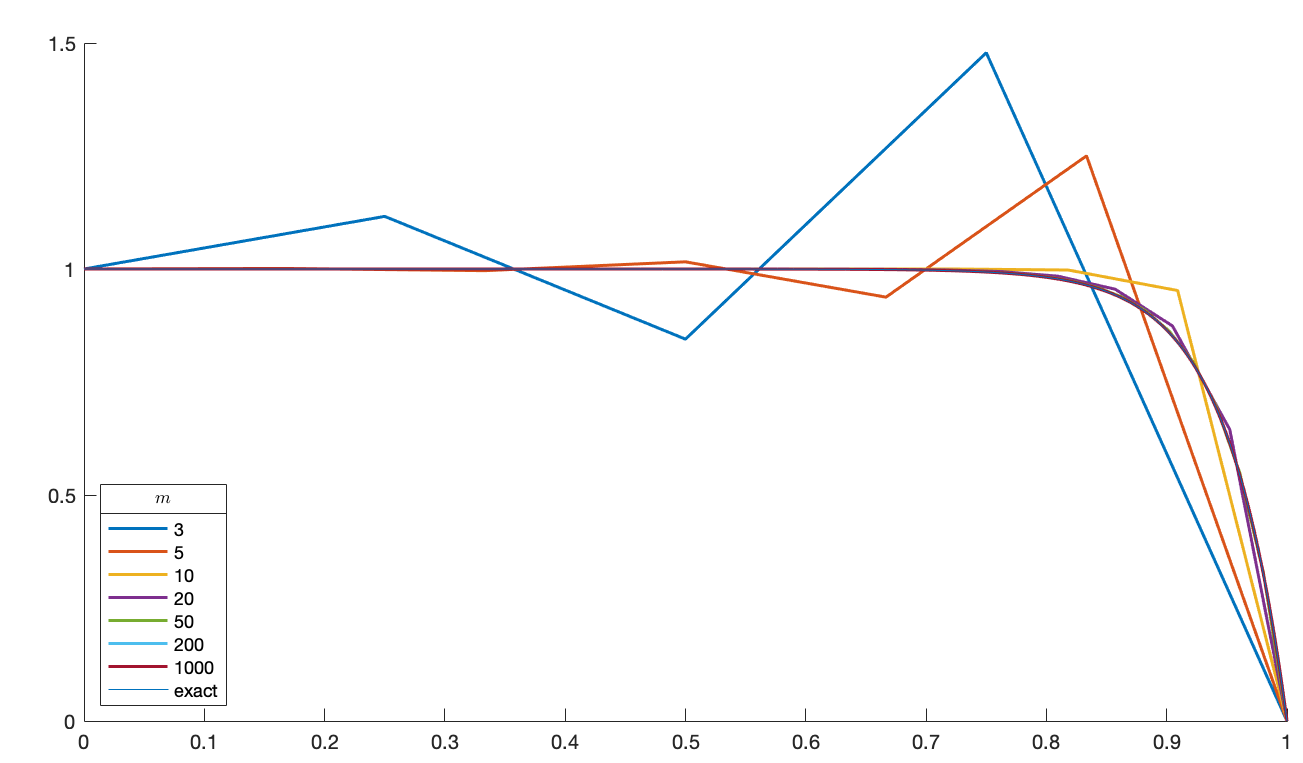
\includegraphics[width=\textwidth]{figP20.png}
    \end{center}
  \end{figure}
  
  
  \textbf{Console:}
  \begin{center}
    \lstinputlisting[basicstyle = \footnotesize]{r8.txt}
  \end{center}

  \item[(c)] Observe that the solutions for small values of $m$ are poor but the high $m$ solutions all basically agree. Why do you think that 
  small $m$ values are problematic here, though they are not for the problem solved in section 2.4? Write a few sentences, perhaps based on a 
  bit of research into Section 2.17. 
  \solution This behavior where small $m$ values are a problem seems to be cause by a rapidly changing solution over a very small interval. Naturally 
  increasing the number of sample points in order to capture that change seems to fix the problem. Our text describes this as a singular perturbation problem. In this second order case we have 
  a problem of the form $-\kappa u''(x) + au'(x) = f(x)$, noting it is equivalent to $\epsilon u''(x) - u'(x) = f(x)$ where $\epsilon = \kappa/a$. When $a$ is sufficiently large relative to $\kappa$,
  $\epsilon$ approaches 0 and the problem can be thought of as a small perturbation to the first order $-u'(x) = f(x)$. In our problem this happens near the $u(1) = 0$ boundary. Here the derivatives of $u(x)$
  are very large and since our centered FD schemes for $u'$ and $u''$ are proportional to $h^2u'''(x)$ and $h^2u''''(x)$ respectively. Without sufficiently small $h$ we can expect the error to be very large. 


\end{exercise}
\vspace{1in}





\begin{exercise}{Proeblem P21} 
  \begin{enumerate}
    \item[(a)] Based on the ideas in sections 3.1-3.3, namely centered finite differences, write a matlab code that 
    solves the Poisson equation on the unit square $0 \leq x \leq 1$, $0 \leq 1$, with zero Dirichlet boundary conditions. Allow 
    the user to set the function $f = f(x, y)$. 
    \solution Slightly modifying heat.m we solve this problem with Dirichlet conditions instead. \\
      
  \textbf{Code:}
  \begin{center}
    \lstinputlisting[basicstyle = \footnotesize]{r9.txt}
  \end{center}


  \item[(b)] Find an appropriate nonzero exact solution that allows you to verify that the code converges at the theoretically-exprected
  rate. That is, show that $||E^h||_2 \to 0$, as $h \to 0$, at the rate $O(h^2)$ if $\Delta x = \Delta y = h = 1/(m + 1)$. 
  \solution Consider the following function which satisfies the Dirichlet boundary conditions, 
  \begin{equation*}
    u(x) = x(1 - x)sin(\pi x).
  \end{equation*}
  Solving for the second partial derivatives found in the poisson equation we get, 
  \begin{equation*}
    u_{xx} = -2\sin \left(\pi y\right),
  \end{equation*}
  \begin{equation*}
    u_{yy} = -\pi ^2x\sin \left(\pi y\right)\left(1-x\right).
  \end{equation*}
  Using the testheat2d.m code we can quickly use grid refinements to check convergence via the discrete $L^2$ Norm. Doing so we find that the code converges 
  converges to the theoretical rate of $O(h^2)$. 
     
  \begin{figure}[H]
    \begin{center}
      \caption{Convergence Plot via Discrete $L^2$ Norm}
      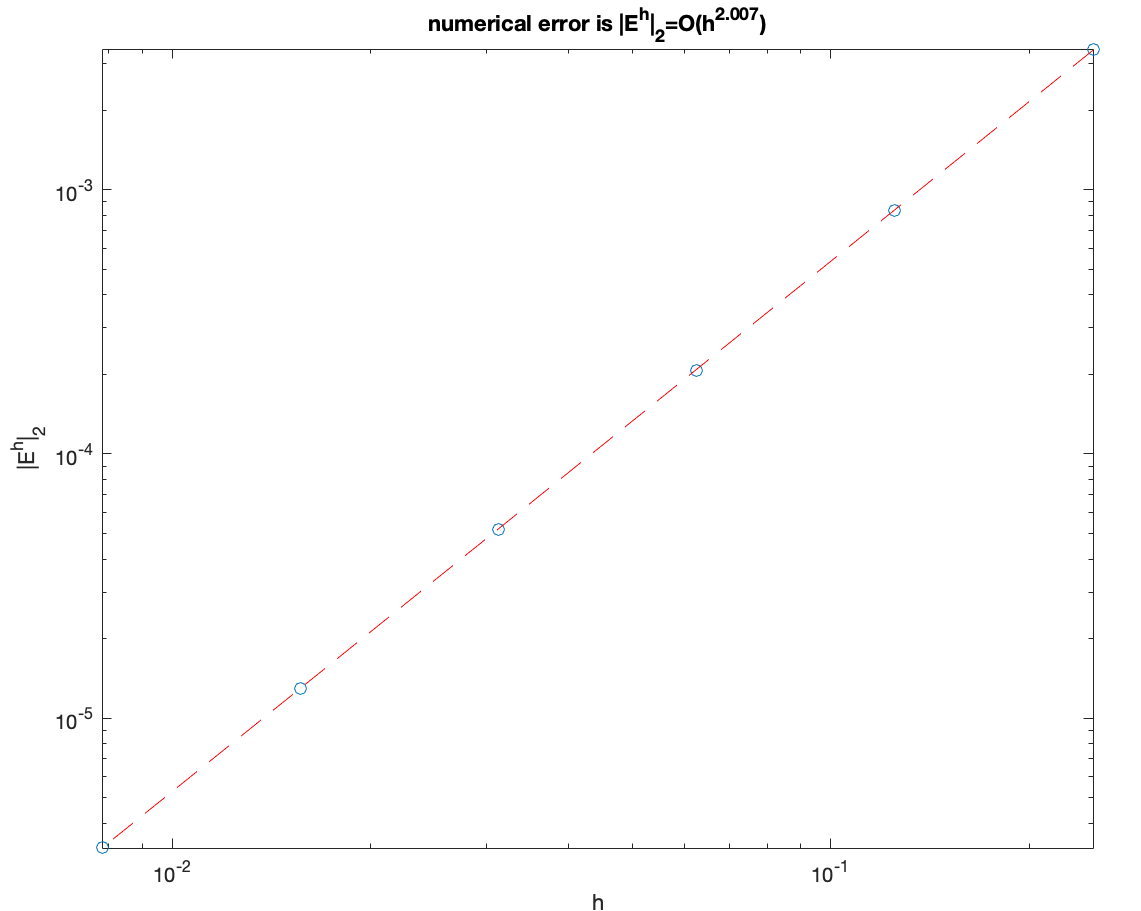
\includegraphics[width=\textwidth]{convergence2d.png}
    \end{center}
  \end{figure}

  \item[(c)] Use Matlab's spy, or similar, to show the sparsity pattern of the matrix $A^h$ for $m = 5$. Also confirm in that case that the matrix
  has the form shown by equation (3.12). 
  \solution Running our modified heat.m with poisson equation defined in the previous part with $m = 5$ we get the following spy plot, 


  \begin{figure}[H]
    \begin{center}
      \caption{Spy Plot $m = 5$.}
      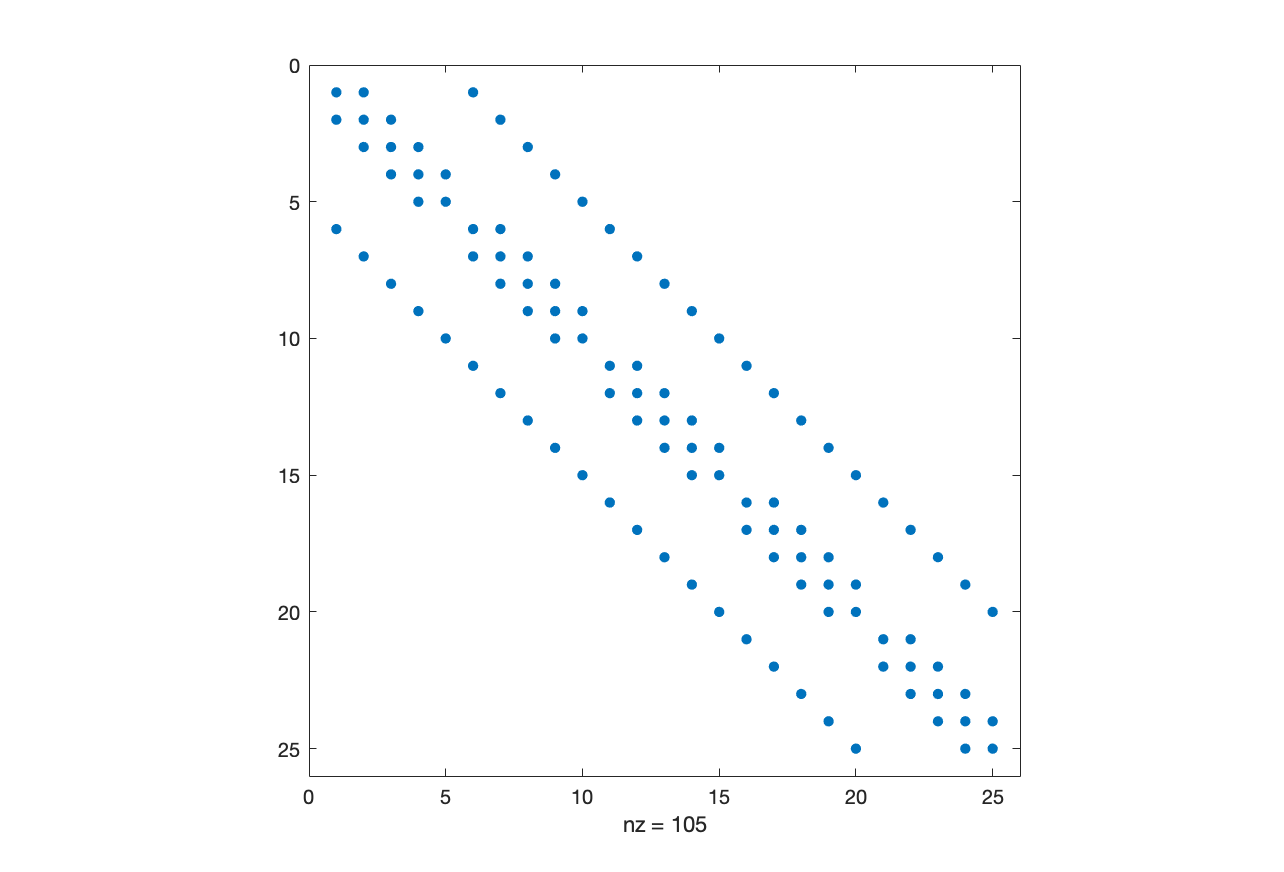
\includegraphics[width=\textwidth]{spy.png}
    \end{center}
  \end{figure}
  This is as expected, and follows the tridiagonal block structure described in equation 3.12 of the text. 



  \end{enumerate}
  
\end{exercise}


















\end{document}











 




